




















\section{Our model and the training strategy}

The practical goal of our model is to identify \textit{single-hit}s while data
collection is still underway.  From a model perspective, we essentially use the
same neural network architecture to create an experiment-specific \textit{hit} classifier
and a generalized \textit{hit} classifier.  We focus more on explaining how our
experiment-specific classifier works, considering it will have an immediate
impact on real-time classification.  


\subsection{CNN vision backbone}

Our CNN vision backbone consists of two convolutional layers that extract image
features and two fully connected layers that compress these image features into
a low dimensional embedding.  The first convolutional layer uses a $5 \times 5$
single channel filter with a stride of one and no padding.  The second
convolutional layer employs a 32-channel $5 \times 5$ filter with a with a
stride of one and no padding.  A ReLU (rectified linear activation unit)
activation function is applied to the outcome of each convolutional layer, which
is followed by a max-pooling operation performed by a $2\times 2$ filter with a
stride of two.  Then, two fully connected layer are used to generate the final
embedding with the size of 128.  As a result, all SPI \textit{hit}s are encoded
into embeddings in a latent space, where embedding distance between two
\textit{hit}s, estimated by a squared $L2$ distance, is a measurement of their
similarities.  Theoretically, identically labeled \textit{hit}s should have a
small embedding distance, whereas differently labeled \textit{hit}s should have
a large embedding distance.  

% Maybe discuss how many parameters are involved depending on the image cropping
% and downsizing in data preprocess.  

%% row x col x filters
%% \renewcommand{\arraystretch}{1.4}
%% pnCCD: 
\begin{table}
\caption{

    The architecture of the CNN vision backbone.  We only specify architectural
    parameters that are independent of input image dimensions.  The benefit is
    that those parameters can be readily used in machine learning frameworks,
    such as PyTorch or Tensorflow.  The exact value of $*$ in the layer ``FC 3"
    depends on the input image size, and can be figured out during the
    initialization of the network.  

}
%% \resizebox{1.0\textwidth}{!}{
    \begin{tabularx}{\textwidth}{   l | l l X X X  }
        Layer       &  In channels    & Out channels    & Kernel size & Stride       & Padding     \\
        \hline
        Conv 1      &  1              & 32              & 5           & 1            & 0           \\
        ReLU 1      &  \textemdash    & \textemdash     & \textemdash & \textemdash  & \textemdash \\
        MaxPool2D 1 &  \textemdash    & \textemdash     & 2           & 2            & 0           \\
        Dropout 1   &  \textemdash    & \textemdash     & \textemdash & \textemdash  & \textemdash \\
        \hline
        Conv 2      &  32             & 64              & 5           & 1            & 0           \\
        ReLU 2      &  \textemdash    & \textemdash     & \textemdash & \textemdash  & \textemdash \\
        MaxPool2D 2 &  \textemdash    & \textemdash     & 2           & 2            & 0           \\
        Dropout 2   &  \textemdash    & \textemdash     & \textemdash & \textemdash  & \textemdash \\
        \hline
        \hline
        Layer       &  In features    & Out features    & \textemdash & \textemdash  & \textemdash \\
        \hline
        FC 3        &  *              & 512             & \textemdash & \textemdash  & \textemdash \\
        ReLU 3      &  \textemdash    & \textemdash     & \textemdash & \textemdash  & \textemdash \\
        \hline
        FC 4        &  512            & 128             & \textemdash & \textemdash  & \textemdash \\
    \end{tabularx}
%% }
\end{table}


\subsection{Triplet loss function for training}

How to train the CNN vision backbone to distinguish SPI \textit{hit}s?  We use a strategy
adopted from FaceNet \cite{schroffFaceNetUnifiedEmbedding2015} that uses a
triplet loss function for training the vision backbone.  Each input consists of
a triplet of SPI \textit{hit}s, which are called an anchor $x^a$, a positive $x^p$ and a
negative $x^n$. The anchor shares the same label as the positive but different
from the negative.  Two pairs will be put into a comparison in the model. The
postive pair contains the anchor and the positive $(x^a, x^p)$, whereas the
negative pair include the anchor and the negative $(x^a, x^n)$.  During training,
three identical CNNs $f$ extract features from a triplet $(x^a, x^p, x^n)$,
while another component in the model measures the squared $L2$ distance in the
positive pair $\|f(x^a) - f(x^p)\|_2^2$ and the negative pair $\|f(x^a) - f(x^n)
\|_2^2$, respectively.  The objective of training our CNN $f$ is to separate the
negative pair $(f(x^a), f(x^n))$ more than the the positive pair $(f(x^a),
f(x^p))$ by at least a margin of $\alpha$.  Suppose there are $N$ triplets, the
objective can be stated as 

\newcommand{\isep}{\mathrel{{.}\,{.}}\nobreak}
\begin{equation} \label{eq:objective}
    \begin{array}{l}
       \|f(x_i^a) - f(x_i^p)\|_2^2 + \alpha < \|f(x_i^a) - f(x_i^n)\|_2^2, \, i = 1 \isep N
    \end{array}
\end{equation}

Meanwhile, we enforce that every embedding has a unit length of one in a
$d$-dimensional latent space, namely $f(x) \in \mathbb{R}^d$ and $\|f(x)
\|_2=1$. It means that a \textit{hit} will be mapped to a single point on a
$d$-dimensional hypersphere with a radius of one.  We can expect identically
labeled \textit{hit}s will get closer over the course of training and eventually
form a cluster.  The average distance between two clusters will ideally be
$\alpha$ in a squared $L2$ norm sense. The largest value of a possible $\alpha$
is 4. Since we consider only three classes, there is plenty of room to fit them
on a hypersphere.  As a result, the value of $\alpha$ can take on many values.
FaceNet choose a very small $\alpha$ because they need to fit millions of
classes onto a hypersphere and clusters have to sit close to one another.  

To facilite the training, the objective in Eq. (\ref{eq:objective}) is turned into the
triplet loss function in Eq. (\ref{eq:triplet_loss}).

\begin{equation} \label{eq:triplet_loss}
    \sum_{i=1}^{N} \left[ \alpha + \|f(x_i^a) - f(x_i^p)\|_2^2 - \|f(x_i^a) -
    f(x_i^n)\|_2^2 \right]_+
\end{equation}

where $[\cdot]_+$ returns zero unless the input value is positive.  


\subsection{Selection of semi-hard triplets}

A triplet can be drawn completely randomly in three steps: (1) Randomly choose
one class;  (2) Randomly sample two examples from the chosen class;  (3)
Randomly sample one example from any class other than the chosen class.  This
method, despite being easy to implement, might not deliver fast convergence when
there are many easy triplets.  We consider three kinds of triplets that might
exist during model training: easy, semi-hard and hard shown in Fig. \ref{fig:
semi-hard}.  In an easy triplet, the negative example is already separated by at
at least a margin of $\alpha$ than the positive example.  In a hard triplet, the
negative example is actually closer to the anchor than the positive is.  In a
semi-hard triplet, the negative example still stays more apart from the anchor
than the positive example does, but the margin is smaller than $\alpha$.  The
problem with easy triplets is that they contribute to zero in the triplet loss,
and thus the training adjusts the model weights according to other triplets. The
problem with too many hard examples is that hard examples are more likely to be
from a small fraction of samples, and minimization routine will prioritize the
separation of those few hard examples from the anchor, which can lead to bad
local minima.  Therefore, it's a more reasonable option to select semi-hard
triplets for training.  This strategy doesn't mean to ignore hard examples at
all.  Instead, once hard examples are pulled into the semi-hard zone,
minimization can eventually pull them into the easy zone. This way allows
majority of the negative examples to stay away from the anchor by a considerable
margin $\alpha$.  From a practical standpoint, the selection of semi-hard
triplets is done at the mini-batch level, where our model randomly selects a
triplet that satisfies the following condition.  

\begin{equation}\label{eq: semi-hard condition}
    \begin{aligned}[b]
    &\|f(x_i^a) - f(x_i^p)\|_2^2 \;<\; \|f(x_i^a) - f(x_i^n)\|_2^2 \;<\;
    \|f(x_i^a) - f(x_i^p)\|_2^2 + \alpha, \\
    &i = 1 \isep N
    \end{aligned}
\end{equation}

\begin{figure} 
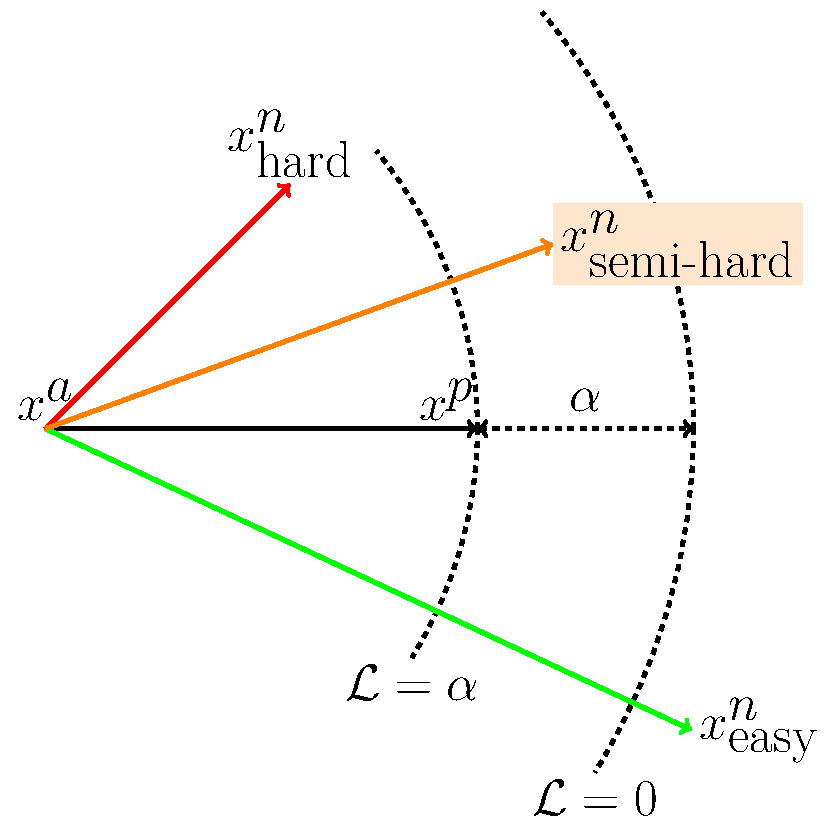
\includegraphics[width=1.0\textwidth,keepaspectratio]
{./figures/triplet.semihard.pdf} 
\caption{

    An illustration of three types of negative examples.  $x^a$ represents an
    anchor example and $x^p$ is a positive example.  Two arcs in dashed lines,
    both centered at $x^a$, are used to divide the 2D plane into three areas.
    The inner arc has a radius of $\|f(x_i^a) - f(x_i^p)\|_2^2$, whereas the
    outer arc has a radius that is larger by a margin of $\alpha$.  Negative
    examples will possess three difficult levels in model training based on the
    area where they are situated.  It's considered as a hard negative example if
    it's located within the inner arc, where $\|f(x_i^a) - f(x_i^n)\|_2^2 <
    \|f(x_i^a) - f(x_i^p) \|_2^2$.  On the contrary, it's considered as an easy
    negative example when it's goes outside the outer arc, where $\|f(x_i^a) -
    f(x_i^n)\|_2^2 - \|f(x_i^a) - f(x_i^p) \|_2^2 > \alpha$.  Lastly, it becomes
    a semi-hard negative example when it resides in the area bound between two
    arcs.  Moreover, the loss functions results in $\mathcal{L} = \alpha$ and
    $\mathcal{L} = 0$ when $x^n_{\text{semi-hard}}$ is on the inner arc and
    outer arc, respectively.  Our model training will pull
    $x^n_{\text{semi-hard}}$ close to the outer arc as much as possible, namely
    minimizing the loss.

}
\label{fig: semi-hard} 
\end{figure}


\subsection{Optimization}

We trained our neural network models using Adam
\cite{kingmaAdamMethodStochastic2017} with the learning rate of $10^{-3}$.  The
model weights are initialized to random values from a Gaussian probability
distribution with a mean of $0.0$ and a standard deviation of $0.2$.  


\subsection{Data preprocessing}

We preprocessed SPI \textit{hit}s in our application for three major reasons:
highlight features, upsample datasets and reduce image size.  Firstly, a typical
way to highlight image features is to zoom in on the region of interest (ROI) if
available.  In SPI \textit{hit}s, features are predominantly located near the
X-ray beam center and areas remote to the center have much weaker signals.
Based on this observation, we decide to crop images by only keeping the pixels
in a user-specified ROI.  Secondly, a \textit{hit} collected in a SPI experiment
won't change its nature after an in-plane rotation with the beam path as the
rotational axis.  This feature allows us to upsample our dataset by applying
random in-plane rotations.  It's worth noting that any \textit{hit} class, e.g.
\textit{single-hit}, can have various forms but random rotation cannot alter any
unique form of a class to resemble another one.  Lastly, we downsampled
\textit{hit}s in our dataset by a factor of six if data are collected in pnCCD
panels and two if data are obtained from a simple square detector.  We don't
have an evidence to conclude those values of downsampling would always give the
best trade-off between reducing size and perserving features.  Instead, we found
they offer good enough performances through practices.  

An important caveat of upsampling our dataset is to only perform it after the
dataset is partitioned into training set and test set.  Otherwise, it will lead
to notorious ``data leakage'' issues explained in
\cite{kapoorLeakageReproducibilityCrisis2022}.  A typical consequence of ``data
leakage'' is the delusionally excellent performance of model inference during
testing, where in fact the test set already encompasses upsampled data
``leaked'' from the training set.  In another word, the ``good'' performance is
mostly caused by model memorization or overfitting rather than generalization.


\subsection{Model inference}

Model inference is performed in a \textit{query-against-support} manner.  A
query is a SPI \textit{hit} whose label is to be determined through inference.
In model inference, labeled SPI \textit{hit}s from each class are randomly
sampled to be used as supports.  For example, when working with experimental
data, we use three support \textit{hit}s representing \textit{non-sample-hit},
\textit{single-hit} and \textit{multi-hit}, respectively.  We basically label a
query based on the label of the most similar \textit{hit} found in the support
set.  Similarity is measured by the squared $L2$ distance, which indicates
higher similarity if its value becomes smaller.  Fig.  \ref{fig : model
inference} is an illustration of three queries, demonstrating the labeling of a
\textit{single-hit} (the first row), a \textit{multi-hit} (the second row) and a
\textit{non-sample-hit} (the third row) .  Meanwhile, a parallel method of model
inference is thresholding the distance, which brings about an extra
hyperparameter to tune.  There is no obvious winner as whether
\textit{query-against-support} is consistently better than the threshold method.
However, when the number of unique classes is smaller, e.g.  less than four in
our case, \textit{query-against-support} eliminates a hyperparameter with a
minor trade-off of constructing a support set by sampling labeled \textit{hit}s.
We think the threshold method is a better choice when the number of unique
classes is large, e.g. $\ge 10$.  

\begin{figure}
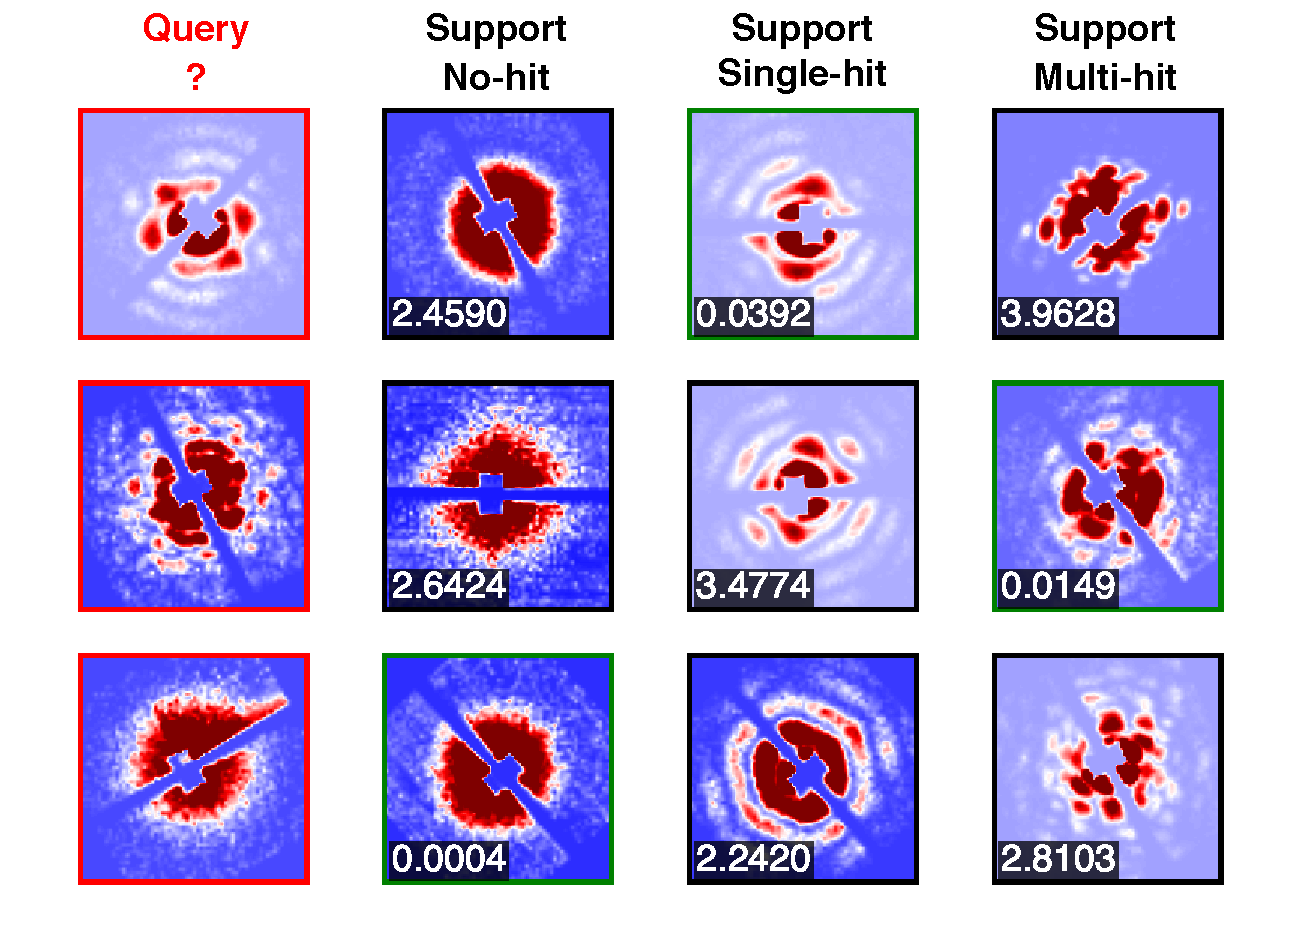
\includegraphics[width=\textwidth,height=0.8\textheight,keepaspectratio]
{./figures/inference.pdf}
\caption{

    An illustration of how the model inference is performed.  Each row
    represents a query against its support.  The predicted label for a query,
    enclosed in a red border, is inferred by the label of the most similar
    support, surrounded by a green border, in a support set, where similarity is
    measured by the squared $L2$ distance between the query and a support.
    Smaller distnace means more similar and vice versa.  

}
\label{fig : model inference}
\end{figure}
